\lstinputlisting[language=bash,basicstyle=\small]{python_codes/fieldstone_71/keywords}

\begin{center}
Code at \url{https://github.com/cedrict/fieldstone/tree/master/python_codes/fieldstone_71}
\end{center}

\par\noindent\rule{\textwidth}{0.4pt}

{\sl This stone was developed in collaboration with Rens Elbertsen}. \index{contributors}{R. Elbertsen}

\par\noindent\rule{\textwidth}{0.4pt}
%%%%%%%%%%%%%%%%%%%%%%%%%%%%%%%%%%%%%%%%%%%%%%%%%%%%%%%%%%%%%%%%%%%%%%%%%%%%%%%%%%%%%%%%%%%%%%

I neeed:
- free slip bc
- max res ?
- crust/lith
- rotated plane 
- compare with submachine


%_____________________________________________________________________________
\subsubsection*{Radial viscosity profiles}

\

In this section we describe the different density profiles used to in the convection model. We assume that viscosity is purely a function of depth. The user can choose a viscosity profile by changing the parameter \texttt{case}.

Five radial viscosity profiles are available:
\begin{itemize}
\item The first viscosity profile is a constant viscosity for all depths of $10^{22}$ Pa s. 
This value is an estimated value of what is normally found in the literature. This is \texttt{visc\_case = 0}. 

\item The second viscosity profile comes from Yoshida et al (2001) \cite{yohk01}. It uses three different regions: lithosphere (0 km to 150 km), upper mantle (150 km to 670 km) and lower mantle (670 km to 2900 km). The function uses an if-statement to return the right value for the given depth. This is \texttt{case = 1}.

\item The third viscosity profile comes from Steinberger \& Holmes (2008) \cite{stho08} 
which is comparable to \cite{stca06}, but of the latter no available data was available. 
Data is read from the file \texttt{visc\_STHO08.dat}. 
This is \texttt{case = 2}.

\item The fourth and fifth profile come from Ciskova et al (2012) \cite{civs12}. 
Data is read from the file \texttt{visc\_CIVS12.dat}. 
The paper showcases two main families of radial viscosity profiles in literature. Family A, which has a sharp 
increase below the 660 km transition zone and remains constant for most of the lower mantle 
and family B which is much smoother over the transition zone and increases with depth in the lower mantle. 
Family A can be chosen by \texttt{case = 3} and family B can be chosen by \texttt{case = 4}.

\end{itemize}

\begin{center}
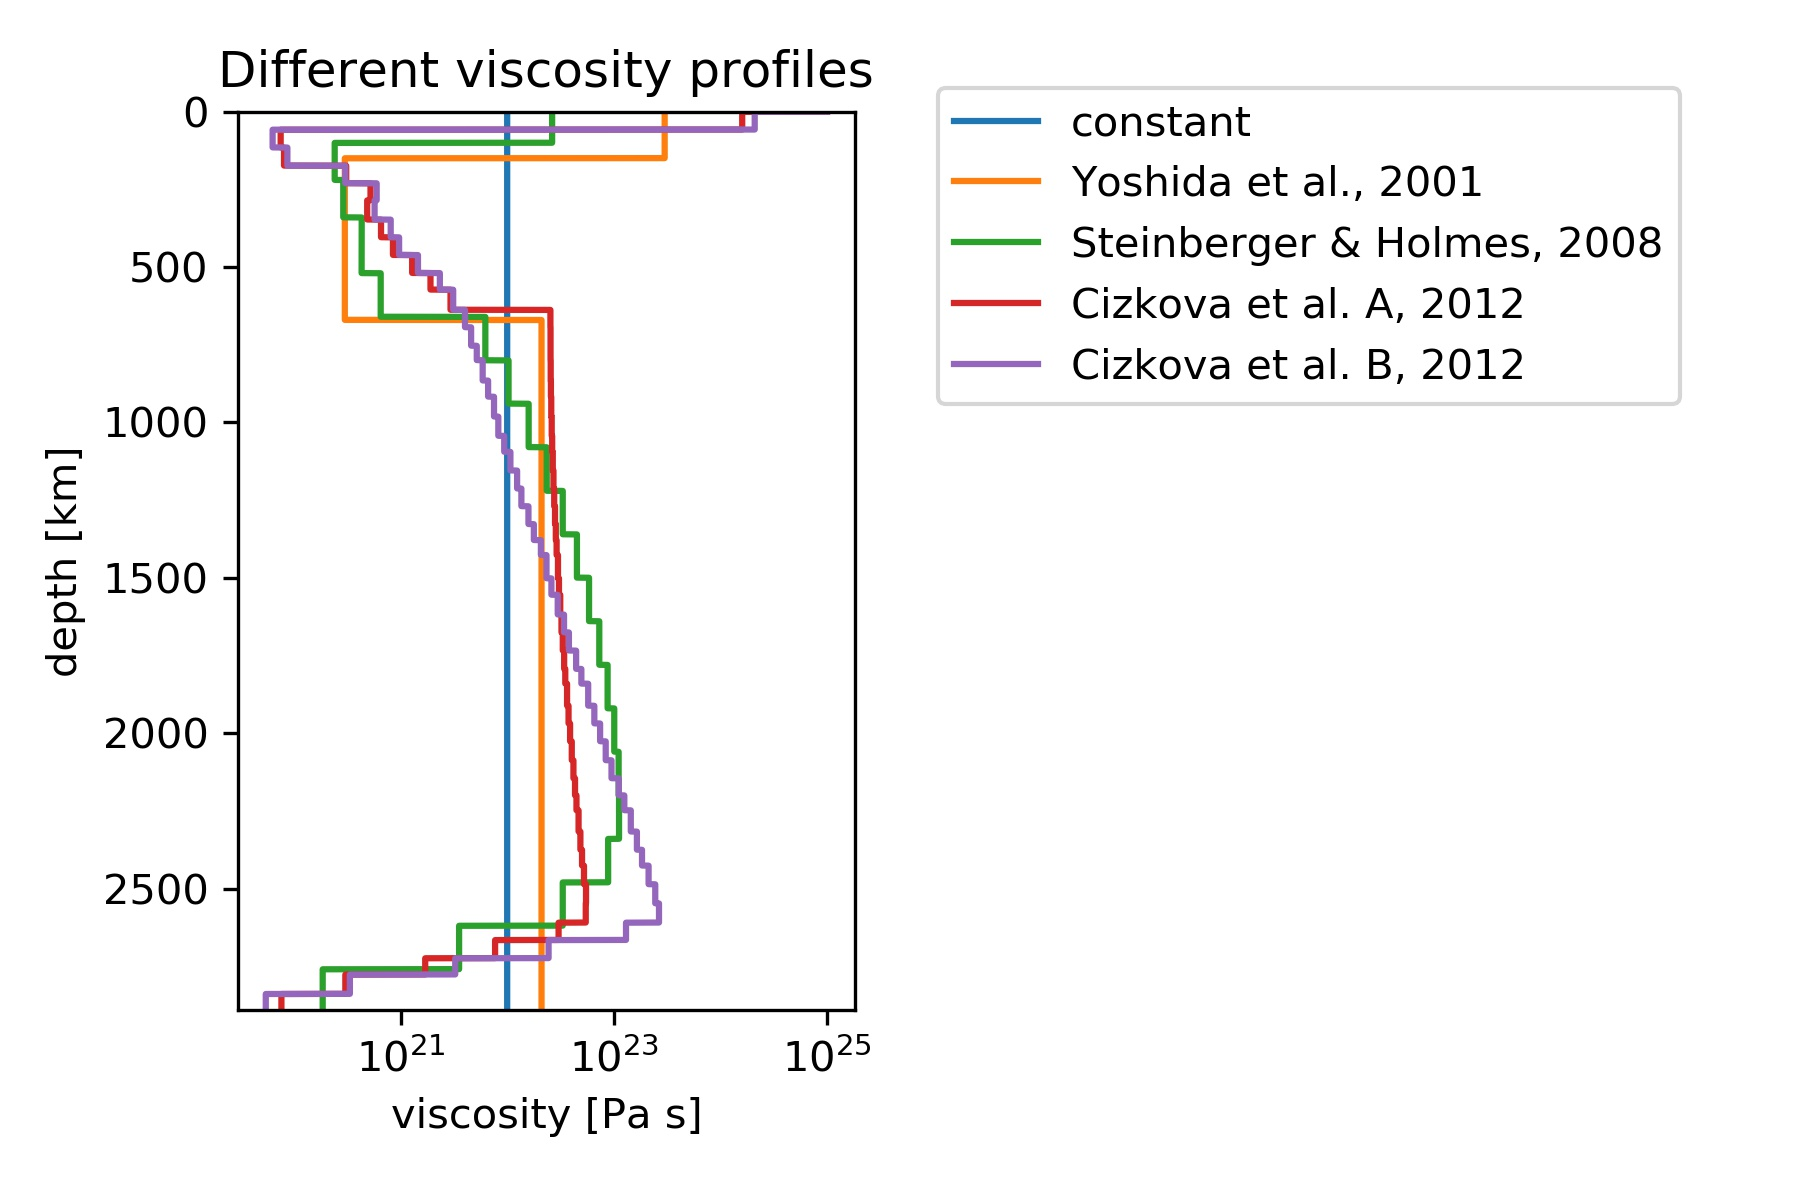
\includegraphics[width=10cm]{python_codes/fieldstone_71/images/visc}
\end{center}


%_____________________________________________________________________________
\subsubsection*{Cross section of the Earth}

Several parameters are implemented which can be modified to get any cross section of the Earth. 

The parameter \texttt{lon\_start} specifies at which longitude we start reading data from the S40RTS model. The model always starts filling the annulus on the right ($x=1, y=0$ on the unit circle) continuing in the counter-clockwise direction with increasing longitudes. If we set the parameter \texttt{plane\_angle} (explained in the next subsection) to 0 we have an equatorial cross section through the Earth that starts at the longitude \texttt{lon\_start}.

The parameter \texttt{plane\_angle} indicates the angle the plane of the cross section is making with the equatorial plane. The longitude specified by \texttt{lon\_start} always is at latitude 0. Latitudes will be increased as a result of the \texttt{plane\_angle} on the northern hemisphere and decreased on the southern hemisphere. Setting the \texttt{plane\_angle} to 90 gives us a cross section through both poles and the longitude specified by \texttt{lon\_start}.



%_____________________________________________________________________________
\subsubsection*{Loading of the Spherical Harmonics, computing $\delta \ln V_s$}

In this stone we wish to use the shear wave velocity model S40RTS \cite{ridv11} 
as the main source of information 
to build a temperature anomaly/density anomaly model of the mantle. 

Variations of the shear wave velocity are stored in the form of spherical harmonics coefficients. 
We make use of an already existing code written by Ross Ronan Maguire
(available at \url{https://github.com/romaguir/sph_models}
to read the values of $d \ln{V_S}$ for a section of the Earth. 
The code is modified such that we read in $d \ln{V_S}$ for every nodal point in the annulus domain. 
Note that the returned value had to be scaled down by a factor of $\sqrt{2}$ to obtain identical figures to 
those of the original paper or those obtained with SubMachine\footnote{\url{https://www.earth.ox.ac.uk/~smachine/cgi/index.php}}.  




There are three different functions in the original code that enables us to read 
the spherical harmonics data: \texttt{read\_splines}, \texttt{read\_sph} 
and \texttt{find\_spl\_vals}. The function \texttt{read\_sph} reads the data from the spherical 
harmonics data file. Thereafter, we loop over all the nodal points. The loop starts at the 
deepest circle of nodes and loops counter-clockwise over this circle before continuing with the 
next circle that is one row of nodal points outwards. The function \texttt{find\_spl\_vals} 
reads the values for a specific depth, meaning that we only have to read these once when we 
start a new circle of nodal points. This function makes use of the other function \texttt{read\_splines}. 
Once we have the correct splines we loop over all nodal points at this depth and calculate the 
value of $\delta \ln{V_s}$ for all these points. The value of $\delta \ln{V_s}$ 
is stored in the array \texttt{d\_ln\_vs}.

\begin{center}
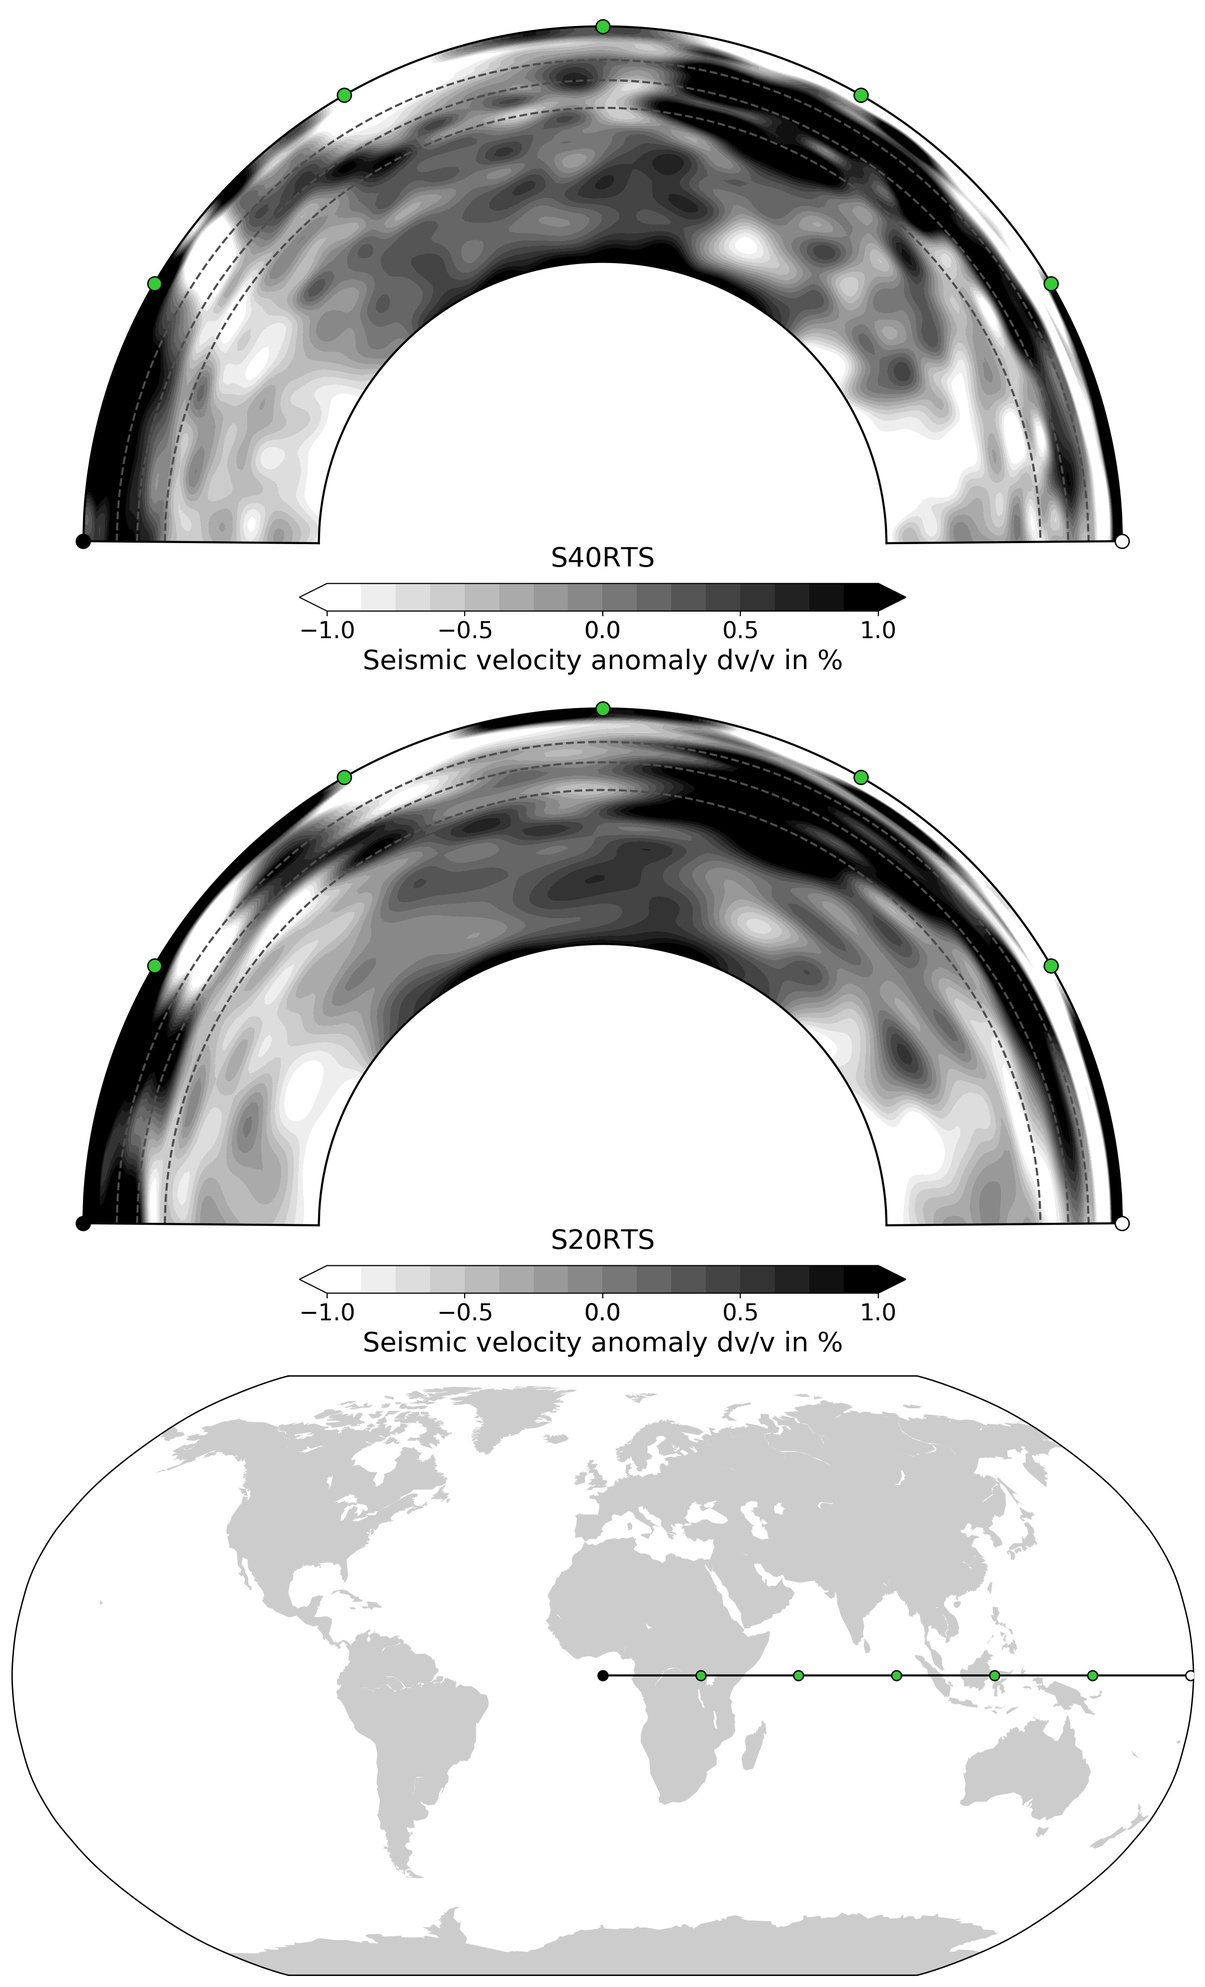
\includegraphics[width=7cm]{python_codes/fieldstone_71/images/sub_cross_section_01}
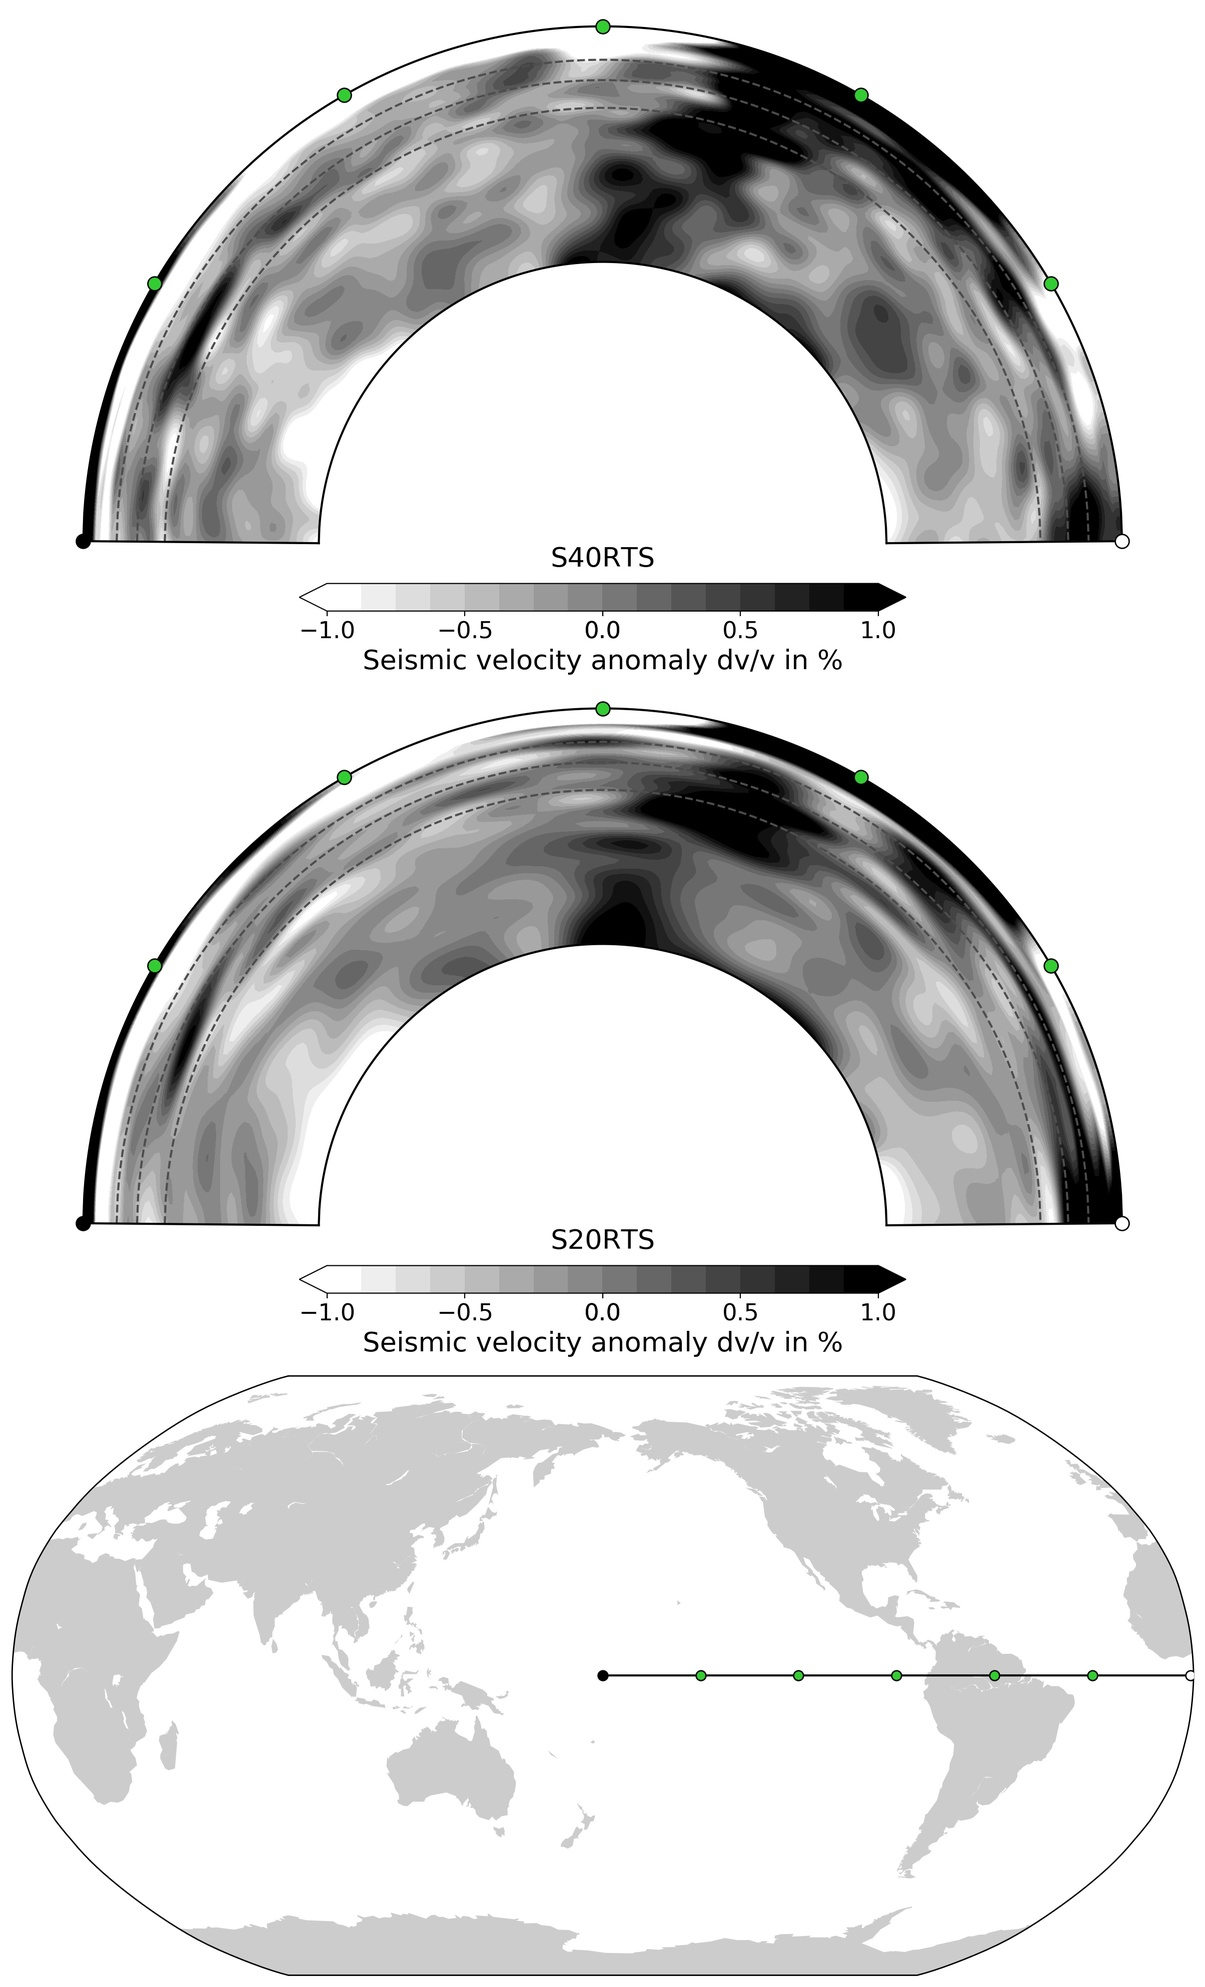
\includegraphics[width=7cm]{python_codes/fieldstone_71/images/sub_cross_section_02}\\
{\captionfont Taken from SubMachine\footnote{\url{https://www.earth.ox.ac.uk/~smachine/cgi/index.php}}.
Cross sections of the mantle for S20RTS and S40RTS models. 
Left: latitude=0, longitude between 0 and 179.
Right: latitude=0, longitude between -179 and 0.}
\end{center}

\begin{center}
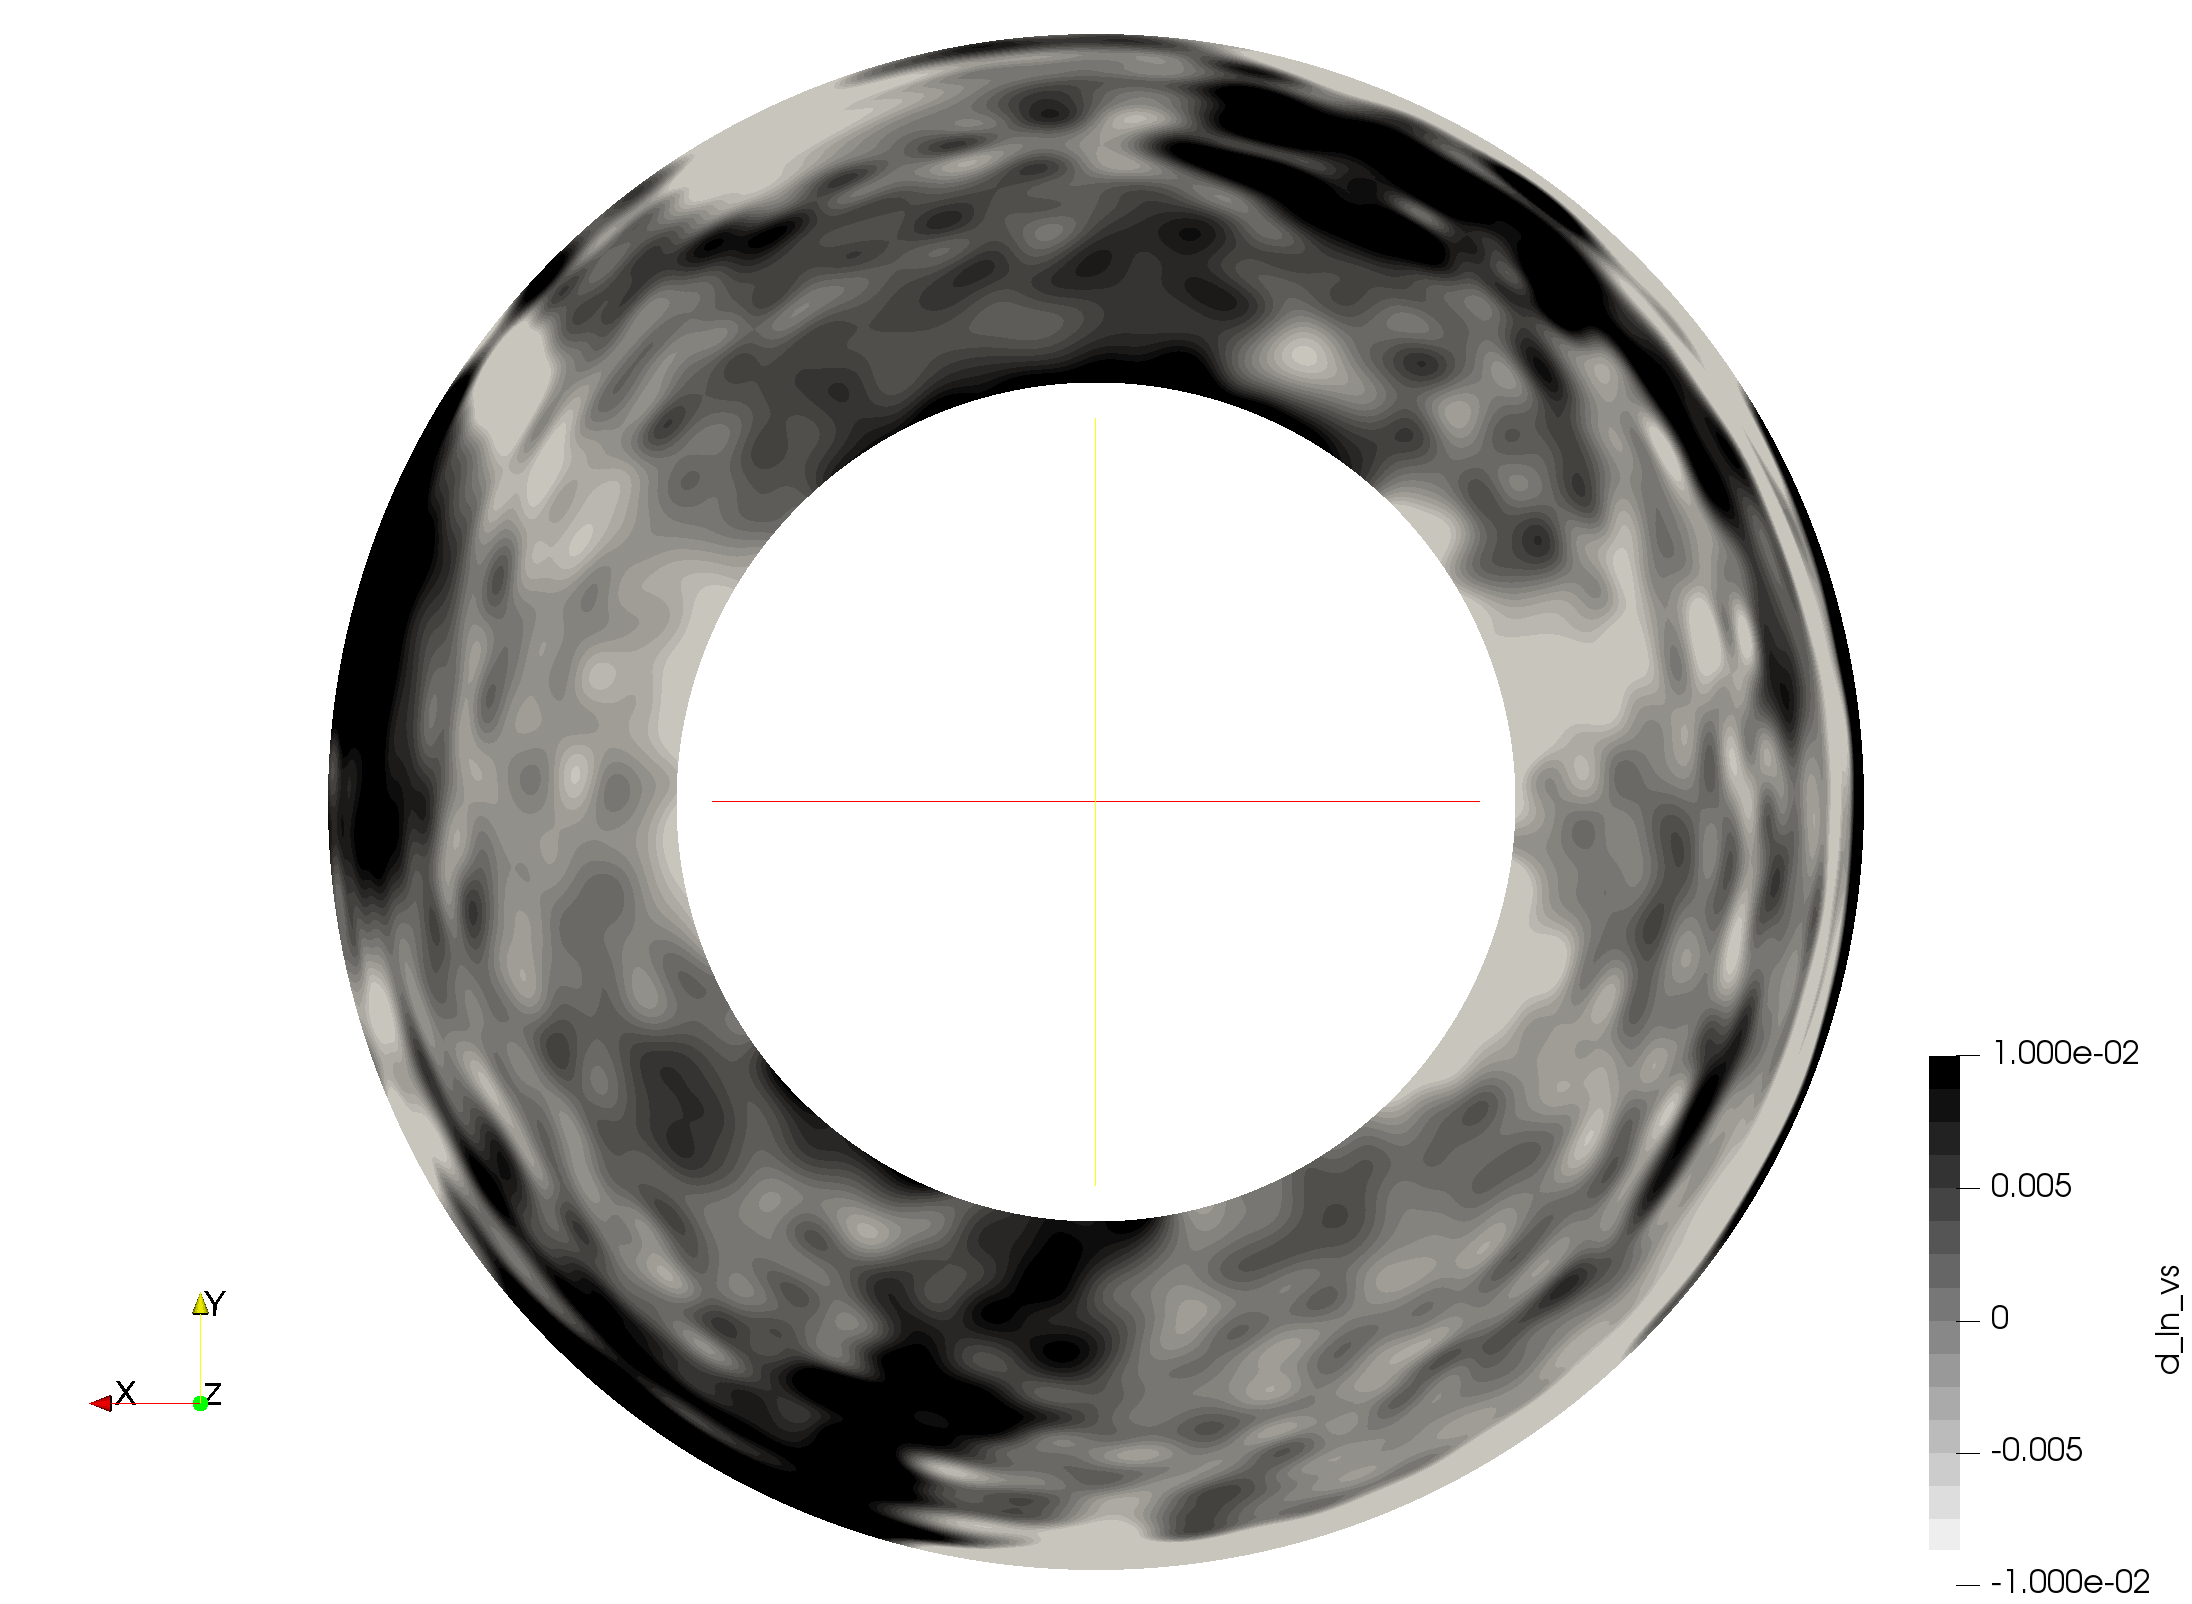
\includegraphics[width=9cm]{python_codes/fieldstone_71/images/dlnvsS40RTS_equator}\\
{\captionfont S40RTS, nelr=50}
\end{center}


%_____________________________________________________________________________
\subsubsection*{Converting $\delta \ln V_s$ to $\delta \rho$}

We assume that there is a direct scaling from the shear wave velocity anomaly to the density anomaly, i.e. 
we assume that all anomalies in $\delta \ln{V_s}$ are the result of temperature perturbations and 
not of differences in composition. 
We use the following formula to obtain the $\delta \ln{\rho} $ values:
\[
\delta \ln{\rho(r, \theta, \phi)} = \xi(r) \cdot \delta \ln{V_s(r, \theta, \phi)} 
\]
where $\xi$ is the scaling factor that is depth dependent. We will go into more depth for this factor in the following subsections. To get the values for $\delta \rho(r, \theta, \phi)$ we use the following formula:
\[
\delta \ln{\rho(r, \theta, \phi)} = \frac{\delta \rho(r, \theta,\phi)}{\rho_\text{ref}} 
\]
where $\rho_\text{ref}$ is the reference density, which in our case for the S40RTS model is the PREM model 
\cite{dzan81}. In the following section we will show which scalings are implemented in the model and how 
they are implemented. The user can choose a scaling by changing the parameter \texttt{xi\_case}. 
The value for $\xi$ is stored in the array \texttt{xi\_nodal}, 
the value for $\rho_\text{PREM}$ is stored in the array \texttt{rho\_prem\_nodal}, 
the value for $\delta \ln{\rho}$ is stored in the array \texttt{d\_ln\_rho\_nodal} 
and the value of $\delta \rho$ is stored in the array \texttt{d\_rho\_nodal}.

There are three options in the code to compute the $\xi$ coefficient:
\begin{itemize}
\item Constant $\xi$. The first scaling that is used is a constant value for $\xi$ of 0.25. 
This is \texttt{xi\_case = 0}. The factor 0.25 is an estimated average of what is normally found in 
literature. An overview of the three different cases can be found hereunder:

\begin{center}
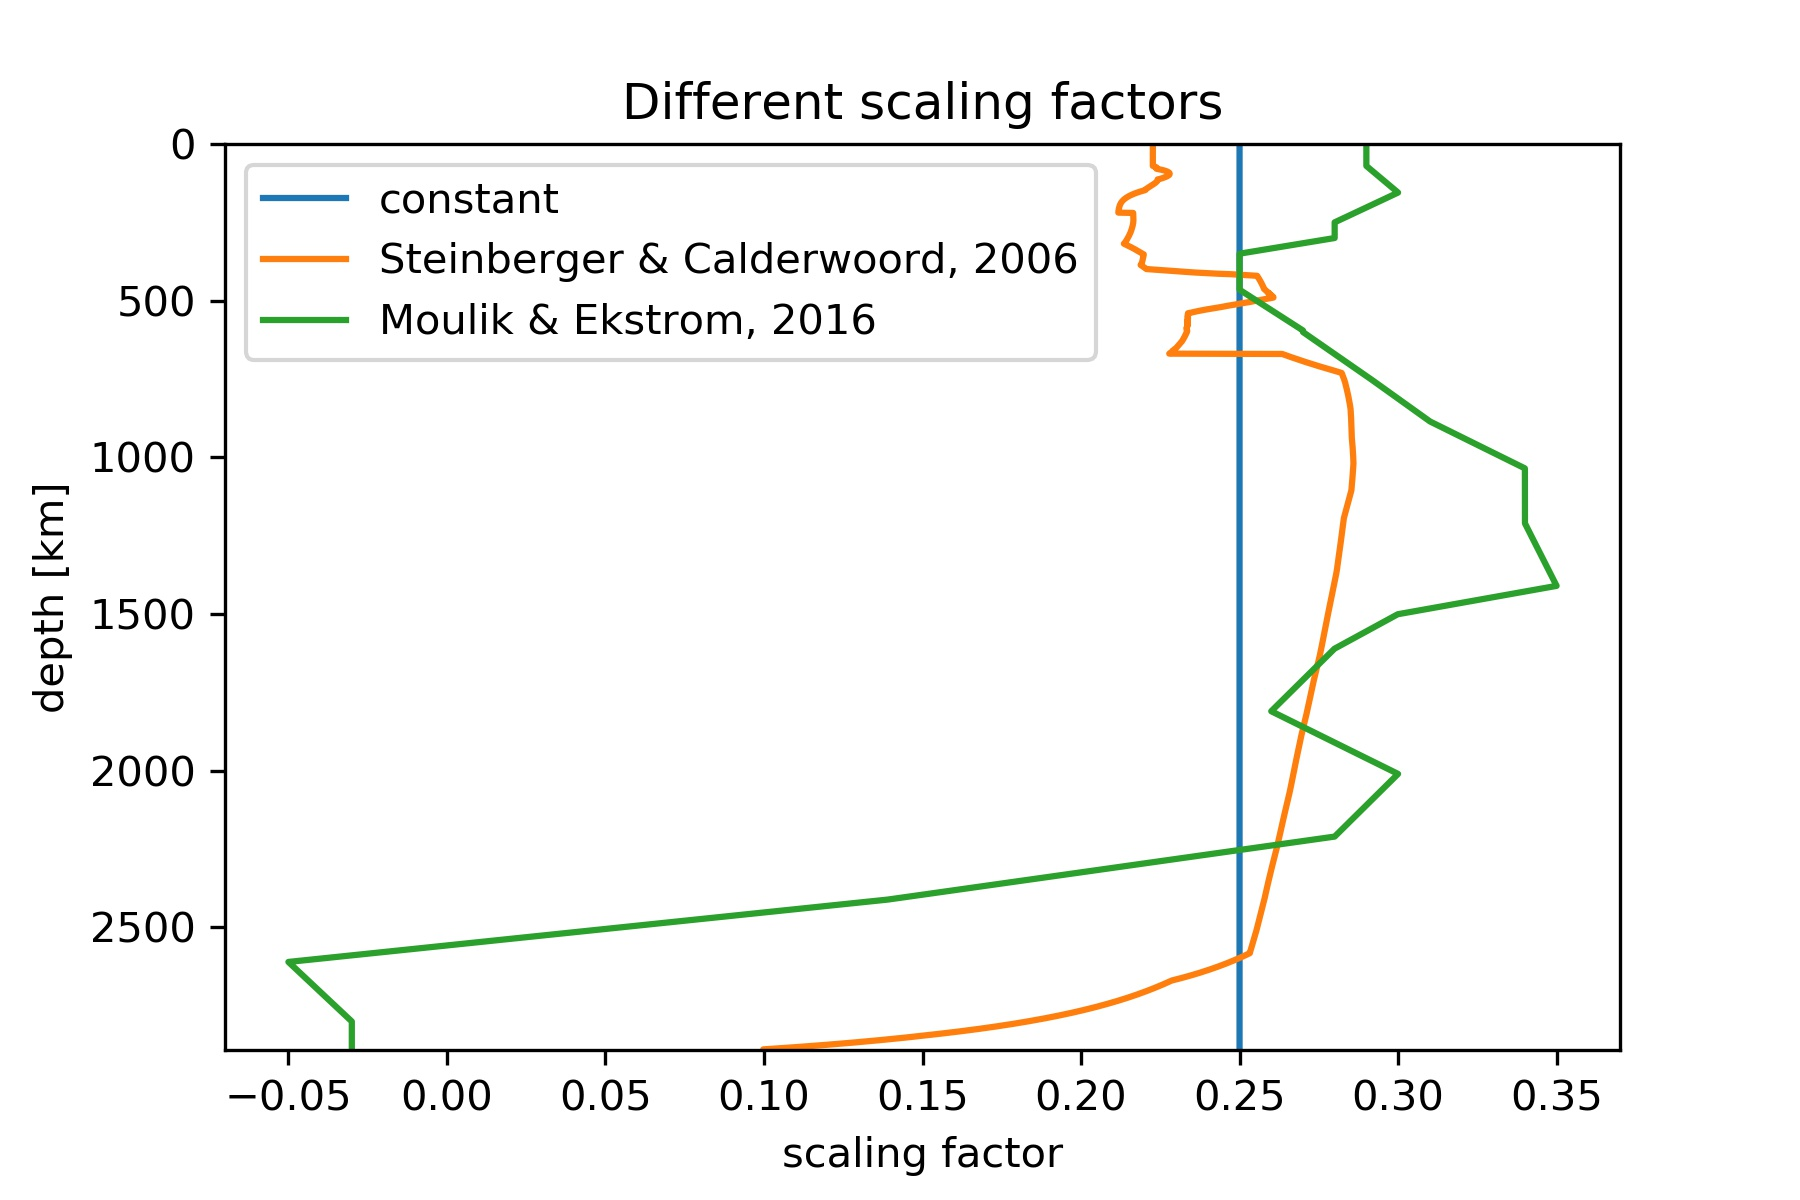
\includegraphics[width=8cm]{python_codes/fieldstone_71/images/xi}
\end{center}

\item The second scaling that is used comes from Steinberger \& Calderwood (2006) \cite{stca06}. 
Data is read from the file \texttt{data/xi/xi\_stca06.ascii}. 

\item The third scaling that is used comes from Moulik \& Ekstrom (2016) \cite{moek16}. 
Data is read from the file \texttt{data/xi/xi\_moek16.ascii}. 
A very noticeable difference between this scaling and the scaling of \cite{stca06} 
is that for the upper mantle the value for $\xi$ is slightly higher and for the lowermost lower mantle 
the value for $\xi$ is negative.
\end{itemize}




